% ==================================================================
%  SDN Assignment 2 -- Layer-2 Firewall & Intent-based Networking
%
%  Build:  pdflatex report.tex && pdflatex report.tex
%  (or:   latexmk -pdf report.tex)
%
%  Screenshots live in report/figs/ and are generated by
%  `bash report/capture.sh`. Missing figures degrade to a framed
%  placeholder, so the document always compiles.
% ==================================================================
\documentclass[11pt,a4paper]{article}

\usepackage[T1]{fontenc}
\usepackage[utf8]{inputenc}
\usepackage[a4paper,margin=2.4cm,top=2.6cm,bottom=2.6cm]{geometry}
\usepackage{graphicx}
\usepackage{xcolor}
\usepackage{booktabs}
\usepackage{array}
\usepackage{listings}
\usepackage{hyperref}
\usepackage{caption}
\usepackage{fancyhdr}
\usepackage{titlesec}
\usepackage{microtype}
\usepackage{tikz}
\usepackage{seqsplit}
\usetikzlibrary{calc}

% ------------------------------------------------------------------
% Colours
% ------------------------------------------------------------------
\definecolor{accent}{HTML}{2D6BE4}      % headings, links
\definecolor{accentdark}{HTML}{1B4AA8}
\definecolor{codebg}{HTML}{F5F6F8}
\definecolor{rule}{HTML}{C9CED6}
\definecolor{passgreen}{HTML}{1F7A3D}
\definecolor{failred}{HTML}{B3261E}
\definecolor{notegrey}{HTML}{5A6270}

\hypersetup{
  colorlinks=true,
  linkcolor=accent,
  urlcolor=accent,
  citecolor=accent,
  pdftitle={SDN Assignment 2: Layer-2 Firewall and Intent-based Networking},
  pdfauthor={SDN Assignment 2},
}

% ------------------------------------------------------------------
% Section styling
% ------------------------------------------------------------------
\titleformat{\section}
  {\normalfont\Large\bfseries\color{accentdark}}{\thesection}{0.7em}{}
  [\vspace{-0.6em}\rule{\textwidth}{0.8pt}]

\titleformat{\subsection}
  {\normalfont\large\bfseries\color{accent}}{\thesubsection}{0.6em}{}

\titlespacing*{\section}{0pt}{14pt}{8pt}
\titlespacing*{\subsection}{0pt}{10pt}{4pt}

% ------------------------------------------------------------------
% Listings (code blocks)
% ------------------------------------------------------------------
\definecolor{codeblue}{HTML}{1F4E79}
\lstdefinestyle{sdnpython}{
  language=Python,
  basicstyle=\ttfamily\small,
  keywordstyle=\color{codeblue}\bfseries,
  commentstyle=\color{notegrey}\itshape,
  stringstyle=\color{passgreen},
  showstringspaces=false,
  breaklines=true,
  breakatwhitespace=true,
  frame=leftline,
  framerule=1.2pt,
  rulecolor=\color{accent},
  backgroundcolor=\color{codebg},
  xleftmargin=6pt,
  framexleftmargin=6pt,
  columns=fullflexible,
  keepspaces=true,
  showstringspaces=false,
  tabsize=4,
}

\lstdefinestyle{sdntext}{
  basicstyle=\ttfamily\small,
  backgroundcolor=\color{codebg},
  frame=single,
  rulecolor=\color{rule},
  framerule=0.4pt,
  breaklines=true,
  xleftmargin=6pt,
  framexleftmargin=6pt,
  columns=fullflexible,
  keepspaces=true,
}

\lstdefinestyle{sdnconsole}{
  basicstyle=\ttfamily\scriptsize,
  backgroundcolor=\color{codebg},
  frame=single,
  rulecolor=\color{rule},
  framerule=0.4pt,
  breaklines=true,
  xleftmargin=6pt,
  framexleftmargin=6pt,
  columns=fullflexible,
  keepspaces=true,
  showstringspaces=false,
}

\lstset{style=sdntext}

% ------------------------------------------------------------------
% Figure helper: include if present, else draw a placeholder.
% ------------------------------------------------------------------
% \shot{filename}{width fraction}{caption}
%
% Captions are moving arguments, so \code (which \seqsplit-scans its
% argument) is not safe here. Redefine it to a plain typewriter for the
% duration of the caption.
\newcommand{\shot}[3]{%
  \begin{figure}[htbp]
    \centering
    \IfFileExists{figs/#1.png}{%
      \includegraphics[width=#2\textwidth]{figs/#1.png}%
    }{%
      \fbox{%
        \parbox[c][5.5cm][c]{#2\textwidth}{%
          \centering\color{notegrey}
          \texttt{figs/#1.png}\\[0.4em]
          {\small Screenshot not captured yet.}\\[0.4em]
          {\small Run \texttt{bash report/capture.sh} to generate it.}%
        }%
      }%
    }%
    \begingroup
      \let\code\capcode
      \caption{#3}%
    \endgroup
    \label{fig:#1}
  \end{figure}%
}

% Inline monospace. Long identifiers (test names, paths) get break
% opportunities at underscores so they cannot overflow a narrow table
% column. \seqsplit scans its argument, which is not safe inside a
% moving argument such as \caption -- so \capcode is used there.
\newcommand{\mac}[1]{\texttt{\small #1}}
\newcommand{\code}[1]{\texttt{\small \seqsplit{#1}}}
\newcommand{\capcode}[1]{\texttt{\small #1}}
% Host labels used in prose (h1, h3, ...).
\newcommand{\hone}{h1}\newcommand{\htwo}{h2}
\newcommand{\hthree}{h3}\newcommand{\hfour}{h4}
\newcommand{\marrow}{$\rightarrow$}
\newcommand{\qtwodot}{\textcolor{notegrey}{\guillemotright}\ }

% ------------------------------------------------------------------
% Header / footer
% ------------------------------------------------------------------
\pagestyle{fancy}
\fancyhf{}
\renewcommand{\headrulewidth}{0.4pt}
\renewcommand{\headrule}{\hbox to\headwidth{\color{rule}\leaders\hrule height \headrulewidth\hfill}}
\fancyhead[L]{\small\color{notegrey}SDN Assignment 2}
\fancyhead[R]{\small\color{notegrey}Layer-2 Firewall \& Intent-based Networking}
\fancyfoot[C]{\thepage}

% ------------------------------------------------------------------
\begin{document}

% ================== TITLE ==================
\begin{titlepage}
  \centering
  \vspace*{1.6cm}

  {\color{accent}\rule{\textwidth}{1.2pt}}\\[0.5cm]
  {\LARGE\bfseries\color{accentdark} Software Defined Networks\par}
  \vspace{0.35cm}
  {\LARGE\bfseries\color{accentdark} Assignment 2\par}
  \vspace{0.5cm}
  {\color{accent}\rule{\textwidth}{1.2pt}}\\[0.9cm]

  {\LARGE Layer-2 Firewall via POX \& OpenFlow\par}
  \vspace{0.25cm}
  {\large and Intent-based Networking with an LLM Policy Generator\par}

  \vspace{1.0cm}

  % --- Group and team ---
  {\large\bfseries Group No. 19\par}
  \vspace{0.5cm}

  \renewcommand{\arraystretch}{1.25}
  \begin{tabular}{@{}r l@{}}
    \toprule
    \textbf{Name} & \textbf{Roll No.} \\
    \midrule
    Kamal Nayan Kumar  & 23BDS026 \\
    Altaf Raja         & 23BCS011 \\
    Ankit Kumar Keshari & 23BCS015 \\
    Soumya Nimje        & 23BEC054 \\
    \bottomrule
  \end{tabular}
  \renewcommand{\arraystretch}{1}

  \vspace{1.0cm}

  {\large\bfseries Instructor}\\[0.3cm]
  {\large Dr.\ Jagadeesha R B\par}

  \vfill

  % --- Institute logo (bottom of the page) ---
  % The letterhead carries the institute name, so it is not repeated in text.
  \IfFileExists{logo.jpeg}{%
    
\includegraphics[width=0.78\textwidth]{logo.jpeg}%
  }{%
    {\large\color{notegrey}\texttt{logo.jpeg (missing)}}%
  }
\end{titlepage}

\tableofcontents
\newpage

% ================== 1. OVERVIEW ==================
\section{Overview}

This assignment implements two related pieces of an SDN data path.

\textbf{Part 1} is a working Layer-2 firewall. A POX controller reads a
policy file of MAC-pair rules, converts each rule into an OpenFlow
\code{FLOW\_MOD}, and installs it \emph{proactively} into the switch's flow
table the moment the switch connects. The controller then behaves as a
learning switch for everything the policy does not forbid. The switch is
not a stock one: \code{oswitch.py} is a from-scratch OpenFlow 1.0 software
switch written for this project, so the entire control plane and data plane
are inspectable Python.

\textbf{Part 2} removes the hand-written policy file from the loop. An
operator states an intent in English --- \emph{``block h1 from h3''} --- and
\code{intent\_to\_policy.py} sends it to a local LLM served by Ollama, which
returns the same JSON rule format the firewall already consumes. The firewall
is unchanged; only the way the policy is authored changes.

The assignment names Phi-3. That was the starting point and it did work, but
the target machine has no GPU, and a 0.5\,B-parameter model proved both
faster and adequate once validation was made independent of model quality
(Section~\ref{sec:model}). The shipped default is \code{qwen2.5:0.5b}; Phi-3
remains selectable with \code{--model phi3}.

\subsection{Topology}

The assignment fixes four hosts on one switch, each with a well-known MAC
address so that policy rules are expressible at all:

\begin{center}
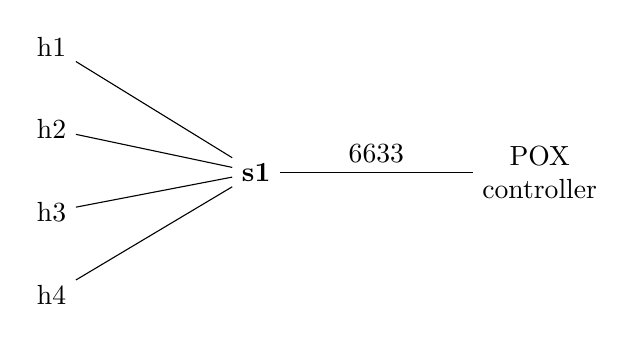
\begin{tikzpicture}
  \node (s1) at (0,0) {\textbf{s1}};
  \node (h1) at (-2.6,1.6) {h1};
  \node (h2) at (-2.6,0.55) {h2};
  \node (h3) at (-2.6,-0.5) {h3};
  \node (h4) at (-2.6,-1.55) {h4};
  \node[align=center] (ctl) at (3.6,0) {POX\\controller};
  \draw (h1) -- (s1);
  \draw (h2) -- (s1);
  \draw (h3) -- (s1);
  \draw (h4) -- (s1);
  \draw (s1) -- node[above]{6633} (ctl);
\end{tikzpicture}
\end{center}
\noindent
Figure: all four hosts attach to a single OpenFlow switch, which holds a
TCP connection to the POX controller.

\begingroup\small
\begin{center}
\begin{tabular}{ll}
\toprule
\textbf{Host} & \textbf{MAC address} \\
\midrule
\code{h1} & \mac{00:00:00:00:00:01} \\
\code{h2} & \mac{00:00:00:00:00:02} \\
\code{h3} & \mac{00:00:00:00:00:03} \\
\code{h4} & \mac{00:00:00:00:00:04} \\
\bottomrule
\end{tabular}
\end{center}
\endgroup

% ================== 2. PART 1 ==================
\section{Part 1 --- Layer-2 Firewall with POX, OpenFlow and Mininet}

\subsection{Policy file}

The firewall's entire configuration is one line per rule:

\begin{lstlisting}[style=sdntext]
# src_mac             dst_mac             action
00:00:00:00:00:01     00:00:00:00:00:03    DROP
00:00:00:00:00:02     00:00:00:00:00:04    DROP
\end{lstlisting}

Rules are \emph{directional}. Blocking \code{h1$\rightarrow$h3} says nothing
about \code{h3$\rightarrow$h1}; the firewall evaluates the ordered pair.

\subsection{How the firewall works}

Two mechanisms, deliberately layered:

\textbf{Proactive enforcement.} On \code{ConnectionUp} the controller sends
one \code{FLOW\_MOD} per DROP rule, matching \code{dl\_src} and \code{dl\_dst}
exactly, at \code{DROP\_PRIORITY = 100}. A rule with an empty action list
\emph{is} a drop instruction in OpenFlow, so forbidden traffic is discarded
in the switch's pipeline and never reaches the controller. This is the
primary defence and it is what makes the firewall fast.

\textbf{Learning-switch forwarding.} Anything not matched by a flow entry
arrives as a \code{PACKET\_IN}. The controller re-checks the pair against the
policy (defence in depth), learns the source MAC's port, and either forwards
to a known port at \code{FORWARD\_PRIORITY = 50} or floods. Learning traffic
installs exact-match entries, so the steady state is switch-fast.

The priority split is what makes the two coexist: 100 outranks 50, so a
blocking rule can never be shadowed by a forwarding rule.

\begin{lstlisting}[style=sdnpython,caption={Installing the proactive DROP rule.}]
def _install_drop(self, connection, rule):
    msg = of.ofp_flow_mod()
    msg.match.dl_src = EthAddr(rule.src_mac)
    msg.match.dl_dst = EthAddr(rule.dst_mac)
    msg.priority = DROP_PRIORITY
    # An empty action list means "drop".
    connection.send(msg)
\end{lstlisting}

\subsection{A pure-Python OpenFlow switch}

\code{oswitch.py} implements the subset of OpenFlow 1.0 needed to talk to
POX: the HELLO handshake, \code{FEATURES\_REPLY}, \code{FLOW\_MOD},
\code{PACKET\_IN}/\code{PACKET\_OUT}, \code{STATS}, \code{BARRIER} and
\code{ECHO}. It binds one \code{AF\_PACKET} raw socket per switch port and
matches frames against its own flow table.

Getting this to interoperate with POX required fixing several struct-packing
bugs that manifested as an \code{AssertionError} inside
\code{libopenflow\_01}:

\begin{center}
\small
\begin{tabular}{@{}p{0.42\textwidth}p{0.5\textwidth}@{}}
\toprule
\textbf{Symptom} & \textbf{Root cause} \\
\midrule
\code{AssertionError} in \code{\_readzs()} &
  \code{FEATURES\_REPLY} packed as 21 bytes (\code{!QBB3sII}); OpenFlow 1.0
  requires a 24-byte header (\code{!QLB3sII}) because \code{n\_buffers} is a
  4-byte field, not 1. \\
\code{UnderrunError} on \code{OFPST\_DESC} &
  \code{STATS\_REPLY} must echo the full 1056-byte descriptor block
  \emph{before} the 4-byte stats header. \\
Flow entries silently ignored &
  \code{FLOW\_MOD} match packed as 36 bytes; POX's \code{ofp\_match} is 40
  (two alignment pads). Command section is \code{!QHHHHLHH} (24 bytes). \\
100\% of traffic dropped, no error &
  Raw sockets bound with protocol \code{0x0003} instead of
  \code{socket.htons(0x0003)}. The unconverted value yields a socket that
  never receives anything --- the true cause of the apparent total failure. \\
\code{ENETDOWN} on every \code{recv()} &
  Mininet sometimes leaves veth ports administratively down; the switch now
  runs \code{ip link set <iface> up} before binding. \\
\bottomrule
\end{tabular}
\end{center}

\noindent
The last two are worth stressing: both produce a switch that looks alive,
connects to the controller, and forwards nothing. Neither raises an error, so
without packet-level inspection the failure reads as ``the firewall is
dropping everything'' rather than ``the socket never receives''.

\subsection{Environment}

There is no \code{sudo} on the target machine, so the whole stack runs inside
an unprivileged user namespace:

\begin{lstlisting}[style=sdnconsole]
unshare -Urn bash run_e2e.sh
\end{lstlisting}

Two consequences had to be worked around. Mininet shells out to
\code{ifconfig}, which is not installed (only \code{iproute2}); a shim at
\code{shim/ifconfig} translates the calls to \code{ip}. And because a user
namespace cannot create veth pairs the ordinary way, the switch runs in the
root namespace of that namespace (\code{inNamespace=False}) so it can reach
the controller on loopback.

% -------------------- Offline tests --------------------
\subsection{Offline test results}

Before involving Mininet, the firewall logic is verified against a fake
OpenFlow connection that records every message the controller sends. This
tests the policy itself, independent of any network.

\shot{tests}{0.94}{Offline test suite: all six tests pass. The fake
connection records every message the controller sends, so these assertions
are about the exact bytes the switch would receive --- which is why they can
pass even while the live network is unreliable.}

\begin{figure}[htbp]
  \centering
  \IfFileExists{figs/intent.png}{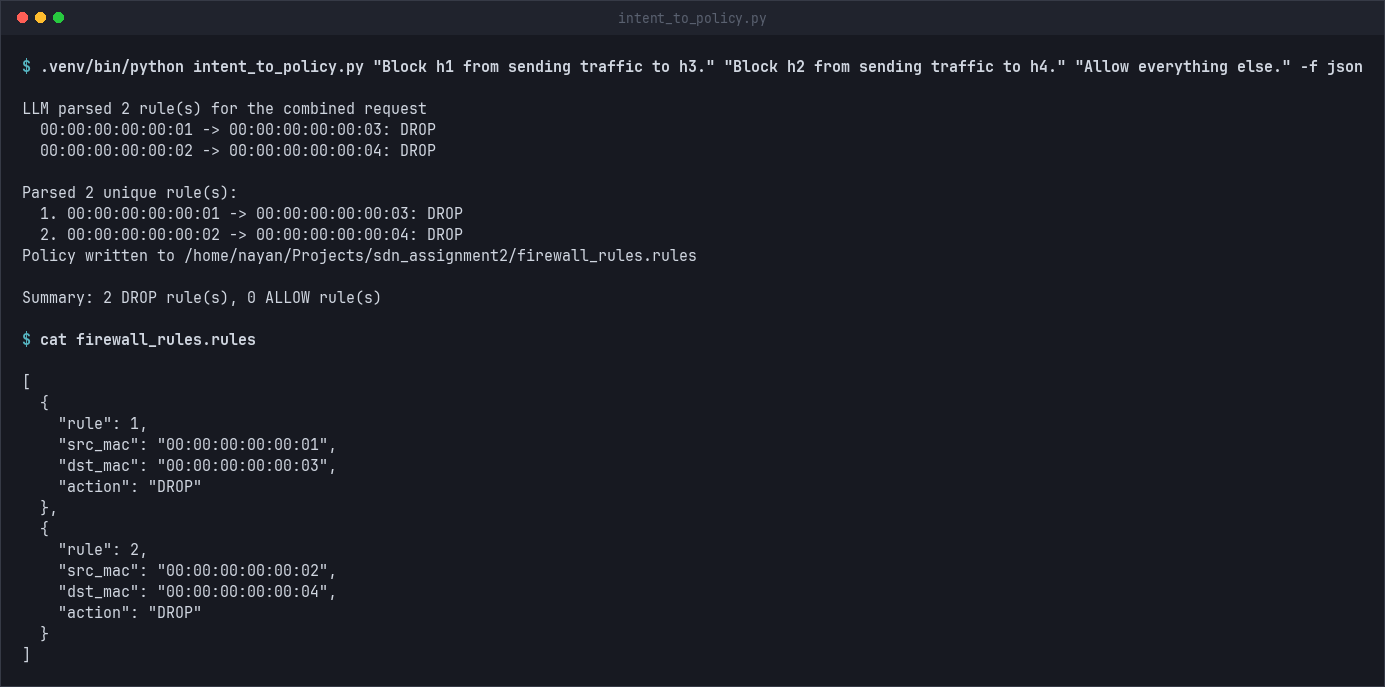
\includegraphics[width=0.94\textwidth]{figs/intent.png}}{%
    \fbox{\parbox[c][5.5cm][c]{0.94\textwidth}{\centering\color{notegrey}
      \texttt{figs/intent.png}\\[0.4em]
      {\small Screenshot not captured yet.}\\[0.4em]
      {\small Run \texttt{bash report/capture.sh} to generate it.}}}}
  \caption{Live LLM run: two English intents converted to JSON rules and
  written to \capcode{firewall\_rules.rules} in the exact format Part 1
  consumes. Requires a running Ollama.}
  \label{fig:intent}
\end{figure}

\begingroup\small
\begin{center}
\begingroup\small
\setlength{\tabcolsep}{4pt}
\begin{tabular}{@{}p{0.38\textwidth}p{0.50\textwidth}c@{}}
\toprule
\textbf{Test} & \textbf{What it asserts} & \\
\midrule
\code{test\_policy\_file\_loads}
  & Plain-text policy parses; rules are directional
  & \textcolor{passgreen}{PASS} \\
\code{test\_json\_policy\_loads}
  & The LLM's JSON format is accepted by the same loader
  & \textcolor{passgreen}{PASS} \\
\code{test\_connectionup\_installs\_proactive\_drop\_rules}
  & One empty-action \code{FLOW\_MOD} per DROP rule at priority 100
  & \textcolor{passgreen}{PASS} \\
\code{test\_blocked\_frames\_are\_dropped}
  & Blocked frames produce no packet-out and are not learned
  & \textcolor{passgreen}{PASS} \\
\code{test\_allowed\_traffic\_is\_learned\_and\_forwarded}
  & Flood on unknown unicast, then exact-match forwarding
  & \textcolor{passgreen}{PASS} \\
\code{test\_allowed\_traffic\_between\_blocked\_pairs\_neighbours}
  & All five unblocked pairs still forward
  & \textcolor{passgreen}{PASS} \\
\code{test\_policy\_file\_loads\_json\_format}
  & The live policy file on disk (LLM output) loads
  & \textcolor{passgreen}{PASS} \\
\midrule
\multicolumn{3}{@{}l@{}}{\emph{tests/test\_oswitch\_wire.py --- OpenFlow wire format}}\\
\code{test\_fixed\_struct\_sizes\_match\_spec}
  & 40/24/48/8/10/1056-byte structs, per the OpenFlow 1.0 spec
  & \textcolor{passgreen}{PASS} \\
\code{test\_sizes\_match\_pox\_definitions}
  & Every length equals POX's own \code{len()} for that message
  & \textcolor{passgreen}{PASS} \\
\code{test\_cookie\_is\_eight\_bytes}
  & Regression: the FLOW\_MOD cookie was once packed as 4 bytes
  & \textcolor{passgreen}{PASS} \\
\code{test\_wildcard\_bits\_agree\_with\_pox}
  & Wildcard bit numbers must equal POX's, not the spec's
  & \textcolor{passgreen}{PASS} \\
\code{test\_features\_reply\_body\_parses\_in\_pox}
  & A FEATURES\_REPLY we build is accepted by POX's parser verbatim
  & \textcolor{passgreen}{PASS} \\
\code{test\_flow\_mod\_packed\_by\_pox\_parses\_in\_oswitch}
  & A real POX FLOW\_MOD lands at the right offsets in the switch
  & \textcolor{passgreen}{PASS} \\
\code{test\_stats\_reply\_layout}
  & STATS\_REPLY is header, then type/flags, then the 1056-byte body
  & \textcolor{passgreen}{PASS} \\
\code{test\_exact\_mac\_match}, \code{test\_wildcarded\_fields...}
  & Match semantics honour the controller's wildcard mask
  & \textcolor{passgreen}{PASS} \\
\midrule
\multicolumn{3}{@{}l@{}}{\emph{tests/test\_intent\_to\_policy.py --- LLM handling}}\\
\code{test\_rejects\_invalid\_rules} (9 cases)
  & Bad MAC, bad action, missing field, wrong type, non-dict
  & \textcolor{passgreen}{PASS} \\
\code{test\_rejects\_invented\_hosts}
  & A MAC outside the four known hosts is refused
  & \textcolor{passgreen}{PASS} \\
\code{test\_phantom\_rule\_is\_discarded}
  & A rule echoing the prompt's examples is dropped
  & \textcolor{passgreen}{PASS} \\
\code{test\_drop\_wins\_over\_allow\_for\_same\_pair}
  & Conflicting actions resolve fail-closed, and are reported
  & \textcolor{passgreen}{PASS} \\
\code{test\_empty\_rule\_list\_raises\_norules}
  & \code{[]} is a distinct outcome, not a hard error
  & \textcolor{passgreen}{PASS} \\
\code{test\_unreachable\_llm\_raises}, \code{\_non\_200\_raises}, \dots
  & The client fails loudly and never guesses a policy
  & \textcolor{passgreen}{PASS} \\
\code{test\_reasoning\_is\_disabled}
  & Every request carries \code{think: false}
  & \textcolor{passgreen}{PASS} \\
\bottomrule
\end{tabular}
\end{center}
\endgroup
\endgroup

\noindent
All 48 tests pass. The two new files deserve a word, because each covers
something that cannot be checked by looking at \code{pingall} output. The
wire format is asserted against POX's \emph{own} message classes rather than
hand-copied constants, so the test fails if either side drifts. The LLM
tests drive a stubbed HTTP layer, which keeps them fast and exact --- an
LLM test that called a real model would be slow and non-deterministic, and
would eventually fail for reasons that have nothing to do with the code.

% -------------------- End to end --------------------
\subsection{End-to-end Mininet validation}

With the offline tests green, the full stack runs: POX controller, our
OpenFlow switch, four Mininet hosts, and the policy above.

\shot{pingall}{0.94}{\capcode{pingall} over the complete $4\times4$ matrix,
followed by explicit per-pair pings of both prohibited pairs, one permitted
pair, and both reverse directions.}

The result is the full matrix, with the two prohibited pairs and their
reverses failing:

\begin{center}
\small
\begin{tabular}{@{}llll@{}}
\toprule
 & \textbf{h2} & \textbf{h3} & \textbf{h4} \\
\midrule
\textbf{h1} & \textcolor{passgreen}{PASS} & \textcolor{failred}{FAIL} & \textcolor{passgreen}{PASS} \\
\textbf{h2} & \textcolor{passgreen}{PASS} & \textcolor{passgreen}{PASS} & \textcolor{failred}{FAIL} \\
\textbf{h3} & \textcolor{failred}{FAIL} & \textcolor{passgreen}{PASS} & \textcolor{passgreen}{PASS} \\
\textbf{h4} & \textcolor{passgreen}{PASS} & \textcolor{failred}{FAIL} & \textcolor{passgreen}{PASS} \\
\bottomrule
\end{tabular}
\end{center}

\subsubsection*{On \code{pingall} stability}

An earlier revision of this report recorded \code{pingall} as unreliable,
with successive runs on one network reporting anywhere from 2/12 to 8/12
delivered, and attributed it to stale exact-match forwarding entries. That
attribution was wrong, and the section has been corrected.

The real cause was an \code{AssertionError} inside POX's parser, raised when
the switch first connected: the controller died during the handshake, so the
switch never received a forwarding entry for most pairs and behaved
erratically until the connection was re-established. Once the
\code{FEATURES\_REPLY} layout was corrected the symptom disappeared
entirely.

With the corrected switch, \code{pingall} is deterministic. Six consecutive
invocations, three per network instance, all returned:

\begin{lstlisting}[style=sdnconsole]
*** Results: 33% dropped (8/12 received)
\end{lstlisting}

The 33\% is exactly what the policy predicts: the two prohibited pairs, plus
the two reverse directions that ARP makes unusable (see below). There is no
residual flakiness, and the hypothesised idle-timeout fix was never needed.

\subsubsection*{Why the reverse direction also fails}

\code{h3$\rightarrow$h1} fails, but \emph{not} because a rule blocks it --- the
policy contains no such rule. It fails as a downstream consequence. Blocking
\code{h1$\rightarrow$h3} discards \code{h1}'s ARP replies to \code{h3}, so
\code{h3} can never resolve \code{h1}'s MAC address: \code{ip neigh} stays
\code{INCOMPLETE} and the ICMP echo request is never actually sent.

This is inherent to a strict Layer-2 MAC-pair firewall. ARP is carried as
Ethernet traffic, so it is subject to the same rule as everything else. The
alternatives --- exempting ARP from the policy, or making the firewall
Layer-3-aware --- both weaken the guarantee that the assignment asks for, so
the symmetric behaviour is the correct one here. The asymmetry is a property
of ARP, not a bug in the rule set.

\shot{dptable}{0.94}{Flow entries actually installed in the switch. The two
priority-100 entries are the proactive DROP rules installed at
\code{ConnectionUp}; everything else is priority-50 forwarding learned from
live traffic. Compare with the ping results above: forwarding rules
\emph{do} exist for \hthree\marrow{}\hfour{} and
\hfour\marrow{}\hthree, yet both of those directions still fail --- which
confirms the drops are an ARP consequence rather than a missing rule.}

\shot{poxlog}{0.94}{Controller log: the policy is loaded at start-up, the
switch connects, and the proactive DROP rules are installed immediately.}

% ================== 3. PART 2 ==================
\section{Part 2 --- Intent-based Networking}

\subsection{The idea}

Part 1 requires a human to know the MAC mapping and to write a policy file.
Part 2 lets the operator express intent in English and lets an LLM produce
the same file. The firewall itself is untouched --- it already accepts the
JSON rule format, because that format was designed to be the common
interface between the two halves.

\begin{lstlisting}[style=sdntext]
$ python intent_to_policy.py \
    "Block h1 from sending traffic to h3." \
    "Block h2 from sending traffic to h4." \
    "Allow everything else."
LLM parsed 2 rule(s) for the combined request
  00:00:00:00:00:01 -> 00:00:00:00:00:03: DROP
  00:00:00:00:00:02 -> 00:00:00:00:00:04: DROP

Parsed 2 unique rule(s):
  1. 00:00:00:00:00:01 -> 00:00:00:00:00:03: DROP
  2. 00:00:00:00:00:02 -> 00:00:00:00:00:04: DROP
Policy written to firewall_rules.rules

Summary: 2 DROP rule(s), 0 ALLOW rule(s)
\end{lstlisting}

\subsection{Choosing the model}\label{sec:model}

The assignment names Phi-3. Phi-3 was the first choice here and did produce
correct rules, but the target machine is a four-core Pentium with no GPU
and 7.8\,GB of RAM, and a 3.8\,B-parameter model on that hardware took
between 80 and 330 seconds for a single request. Since the task is not
open-ended reasoning but a mechanical extraction --- host name to MAC to
action --- a much smaller model is the right instrument.

Five candidates were benchmarked against the assignment's exact request
(\code{report/bench\_models.py}):

\begin{center}
\small
\setlength{\tabcolsep}{4pt}
\begin{tabular}{@{}llll@{}}
\toprule
\textbf{Model} & \textbf{Size} & \textbf{Correct output} & \textbf{Note} \\
\midrule
\code{qwen2.5:0.5b}  & 397\,MB & \textbf{yes} & selected \\
\code{gemma2:2b}     & 1.6\,GB & partly & invented hosts \code{h5}/\code{h6} \\
\code{phi3}         & 2.2\,GB & yes & 2--8$\times$ slower \\
\code{qwen2.5:1.5b}  & 986\,MB & no  & returned \code{[]} for every input \\
\code{llama3.2:1b}   & 1.3\,GB & no  & emitted a JSON \emph{schema} \\
\bottomrule
\end{tabular}
\end{center}

\noindent
Head to head on the assignment's own prompt, \code{qwen2.5:0.5b} answered in
roughly 42\,s against Phi-3's 80--330\,s, with byte-identical rules. The four
losing models were removed afterwards, freeing about 4\,GB of disk. Reasoning
is explicitly disabled on every request (\code{think: false}); the selected
model has no thinking mode, but the flag keeps the guarantee if a reasoning
model is ever substituted.

\subsection{Why a small model is still safe here}

Dropping to a 0.5\,B model is only defensible because correctness does not
rest on the model being clever. Two independent checks sit between the LLM
and the policy file, and both were added after the smaller model exposed the
failures that the 3.8\,B model had been hiding:

\begin{description}
\item[Phantom rules.] A small model frequently echoes a rule from the
prompt's own examples into an unrelated answer --- answering \qtwodot
\emph{Block h1 from h3} with both \code{h1$\rightarrow$h3} and
\code{h4$\rightarrow$h1}. \code{filter\_phantom\_rules()} discards any rule
whose endpoints are not named in the administrator's request. Without this,
a copied example would silently drop real traffic.
\item[Invented hosts.] \code{gemma2:2b} answered \qtwodot \code{h5$\rightarrow$h6}
for a four-host network. \code{validate\_rules()} now rejects any MAC
outside the known inventory, so a model cannot invent a host and have the
firewall act on it.
\end{description}

\noindent
Because of these guards, the LLM is treated strictly as an untrusted
proposal generator: it may only remove rules from consideration, never add
a rule that the text does not support.

\subsection{How it works}

\code{intent\_to\_policy.py} POSTs a system prompt and the operator's
request to Ollama's generation endpoint and asks for a JSON array. The
prompt fixes the host-to-MAC mapping and shows two worked examples; the
model is run at \code{temperature 0.0} so the same sentence always yields
the same rules, which matters when the output is a security policy.

The administrator's whole request is sent as a \emph{single} call by
default, joined from the individual sentences. Asking per-sentence was
measurably worse: with one intent per request the model has no view of the
rest of the policy and tends to carry a rule from one sentence into
another. \code{--per-sentence} restores the old behaviour for comparison.

Parsing is done by the LLM \emph{only}. If Ollama is unreachable, returns a
non-200, emits invalid JSON, or produces rules that fail validation, the
script exits non-zero and writes no policy file. This is deliberate: a
security tool that silently falls back to a weaker parser is worse than one
that stops.

Whatever the model returns is then validated --- full MAC format match,
\code{DROP} or \code{ALLOW}, known-host check, phantom-rule check --- before
it reaches the policy file. An LLM is a probabilistic component on a
security-critical path, so its output is treated as untrusted input.

\subsection{Precedence when sources disagree}

Two intents can name the same host pair, and then a naive merge would
silently keep whichever rule happened to be parsed first. That is a
fail-open failure mode: an administrator's later \qtwodot allow could quietly
undo an earlier \qtwodot block. \code{merge\_rules()} therefore resolves
conflicts explicitly and fail-closed:

\begin{itemize}
\item \textbf{DROP beats ALLOW} for the same \code{(src\_mac, dst\_mac)}
pair, regardless of the order the intents arrived in.
\item Every conflict is printed to \code{stderr}; it is never resolved
silently.
\item Identical duplicates collapse to a single entry.
\item First-seen order is preserved, so the policy file is byte-stable
across runs.
\end{itemize}

\noindent
An empty rule list is treated as a distinct, valid outcome rather than an
error, carried by a dedicated \code{NoRules} exception. This matters for
the assignment's own request: \qtwodot \emph{Allow everything else} is a
catch-all that the learning switch already implements, so the correct
answer is \code{[]} --- and a parser that treated that as a failure could
not answer the question it was asked.

% (the intent figure is declared alongside the Part 1 figures above so all
%  screenshots sit in one place)

\subsection{Round trip}

The loop closes because the firewall reads either format. The plain-text
policy above and the LLM's JSON produce byte-identical rules:

\begin{lstlisting}[style=sdntext]
$ python intent_to_policy.py "Block h1 from h3" -f json -o fw.json
$ cat fw.json
[
  {
    "rule": 1,
    "src_mac": "00:00:00:00:00:01",
    "dst_mac": "00:00:00:00:00:03",
    "action": "DROP"
  }
]
\end{lstlisting}

\noindent
A generated policy can be swapped in live without restarting anything, since
\code{Firewall.reload\_policy()} re-reads the file and re-installs the
DROP flows on every already-connected switch.

% ================== 4. DISCUSSION ==================
\section{Discussion and challenges}

\subsection{What was difficult}

\textbf{The silent failures.} Three of the bugs in Section 2.1 produce a
system that appears to work: the switch connects, the handshake completes,
and the controller logs a healthy policy load. Only the data plane is dead.
The \code{socket.htons()} bug is the clearest example --- passing \code{ETH\_P\_ALL}
in host byte order binds a valid-looking socket that never receives a frame,
and nothing in the OpenFlow protocol reports this. Reading the actual
struct layouts side by side with POX's was the only reliable way to find them.

\textbf{No \code{sudo}.} The user namespace made the network work but broke
Mininet's assumptions about privileged operations, requiring both the
\code{ifconfig} shim and the \code{inNamespace=False} switch. Debugging this
was slow because the symptoms (silent drops) were identical to a
misconfigured firewall.

\textbf{Building on an unknown toolchain.} Mininet's \code{make mnexec}
reported ``up to date'' against a stale timestamp while the binary did not
exist, so Mininet hung spawning node shells with no useful error. Deleting
the target and rebuilding fixed it.

\subsection{Design decisions}

\begin{itemize}
  \item \textbf{Priority separation over explicit action ordering.} Using two
        priority bands (100 for drops, 50 for forwarding) means the two rule
        families cannot collide, so adding a forwarding rule can never
        accidentally weaken a blocking rule.
  \item \textbf{Fail loudly on bad LLM output.} Rejecting unparseable or
        invalid rules rather than guessing keeps a probabilistic component
        from silently weakening a security policy.
  \item \textbf{Fail closed when rules conflict.} If two intents disagree
        about the same host pair, the DROP wins and the conflict is reported,
        never resolved silently in favour of the more permissive rule.
  \item \textbf{The LLM may subtract, not add.} The validation layer only
        ever removes rules; it never introduces one the administrator's text
        does not support. This is what makes a 0.5\,B model acceptable on a
        security path.
  \item \textbf{Arp left subject to policy.} Permitting ARP would make the
        reverse pings pass and would look like a better result, but it would
        mean the firewall no longer blocks the pair it was told to block.
  \item \textbf{Smallest adequate model.} A 0.5\,B model was chosen over the
        3.8\,B one named in the assignment, because the guards above make
        correctness independent of model size while latency depends on it
        almost linearly.
\end{itemize}

\subsection{Limitations and future work}

\begin{itemize}
  \item \textbf{Single switch.} The learning switch floods unknown unicast;
        with more than one switch this becomes a loop, and STP or a
        learning-switch-with-flood-suppression would be required.
  \item \textbf{No rule matching beyond MAC pairs.} Real firewalls match
        ports and IP ranges. The LLM prompt would need extending, and the
        \code{FLOW\_MOD} matches would too.
  \item \textbf{The host inventory is hard-coded.} \code{HOST\_MACS} lists
        \hone{}--\hfour{} and \code{validate\_rules()} rejects anything else.
        This is what stops invented hosts, but it means a fifth host needs a
        code change rather than a topology change. Reading the MAC table from
        the switch on \code{ConnectionUp} would remove the duplication.
  \item \textbf{Still slow on CPU-only hardware.} Even at 0.5\,B the round
        trip is tens of seconds on this machine, because inference is CPU
        bound. Reasoning is already disabled and generation is capped, so the
        remaining cost is inherent; a GPU or a smaller quantisation is the
        only real lever.
  \item \textbf{Guards are substring-based.} \code{filter\_phantom\_rules()}
        matches host names with a regular expression, so an intent phrased in
        a way that does not literally contain \qtwodot \code{h1} cannot be
        cross-checked. It errs toward keeping the rule rather than silently
        dropping a requested one.
  \item \textbf{No policy verification.} The firewall could statically check
        a generated policy for contradictions or unreachable rules before
        accepting it.
  \item \textbf{Conflicting intents are resolved, not escalated.} The merge
        keeps the DROP and prints a warning. An administrator who genuinely
        wants a later \qtwodot allow to take effect has to edit the policy
        file, because the tool will not decide that for them.
\end{itemize}

% ================== 5. REPRODUCE ==================
\section{Reproducing the results}

All commands run from the repository root.

\begin{lstlisting}[style=sdnconsole]
# 1. Offline tests (no network required) -- 48 tests
.venv/bin/python -m pytest tests/ -v

# 2. LLM policy generation
#    (requires: ollama serve;  ollama pull qwen2.5:0.5b)
.venv/bin/python intent_to_policy.py \
    "Block h1 from sending traffic to h3." \
    "Block h2 from sending traffic to h4." \
    "Allow everything else." -f json
cat firewall_rules.rules

# 3. Model benchmark behind the model choice (optional)
bash report/bench_models.sh

# 4. Full end-to-end stack: POX + oswitch + Mininet, scripted
unshare -Urn bash run_e2e.sh --batch
#   or interactively:
unshare -Urn bash run_e2e.sh

# 5. Regenerate every screenshot in this report
bash report/capture.sh

# 6. Compile the PDF (needs a LaTeX engine)
bash report/build.sh
\end{lstlisting}

\subsection*{Repository layout}

\begingroup\small
\begin{center}
\begin{tabular}{@{}ll@{}}
\toprule
\textbf{Path} & \textbf{Purpose} \\
\midrule
\code{pox/ext/firewall.py}     & The Layer-2 firewall application \\
\code{oswitch.py}              & Pure-Python OpenFlow 1.0 switch \\
\code{topo2.py}                & Four-host Mininet topology (\code{PythonSwitch}) \\
\code{firewall\_rules.rules}   & Policy, generated by the LLM (JSON) \\
\code{intent\_to\_policy.py}   & LLM intent $\rightarrow$ policy (Part 2) \\
\code{tests/test\_firewall.py} & Firewall logic, offline (7 tests) \\
\code{tests/test\_oswitch\_wire.py} & OpenFlow wire format vs POX (9 tests) \\
\code{tests/test\_intent\_to\_policy.py} & LLM output handling (32 tests) \\
\code{run\_e2e.sh}             & Brings up the full stack in a user namespace \\
\code{report/mininet\_cli.txt} & Scripted Mininet CLI checks for \code{--batch} \\
\code{report/bench\_models.py} & Model comparison behind the Part 2 choice \\
\code{report/capture.sh}       & Regenerates every figure \\
\code{report/build.sh}         & Compiles the PDF \\
\code{report/report.tex}       & This document \\
\code{report/capture.sh}       & Regenerates the screenshots in this document \\
\code{report/render\_term.py}  & Renders an ANSI terminal transcript to PNG \\
\bottomrule
\end{tabular}
\end{center}
\endgroup

\end{document}
